% CREATED BY DAVID FRISK, 2016
\section{V-REP Models}
\label{app:model}
\begin{figure}[htbp]
    \centering
    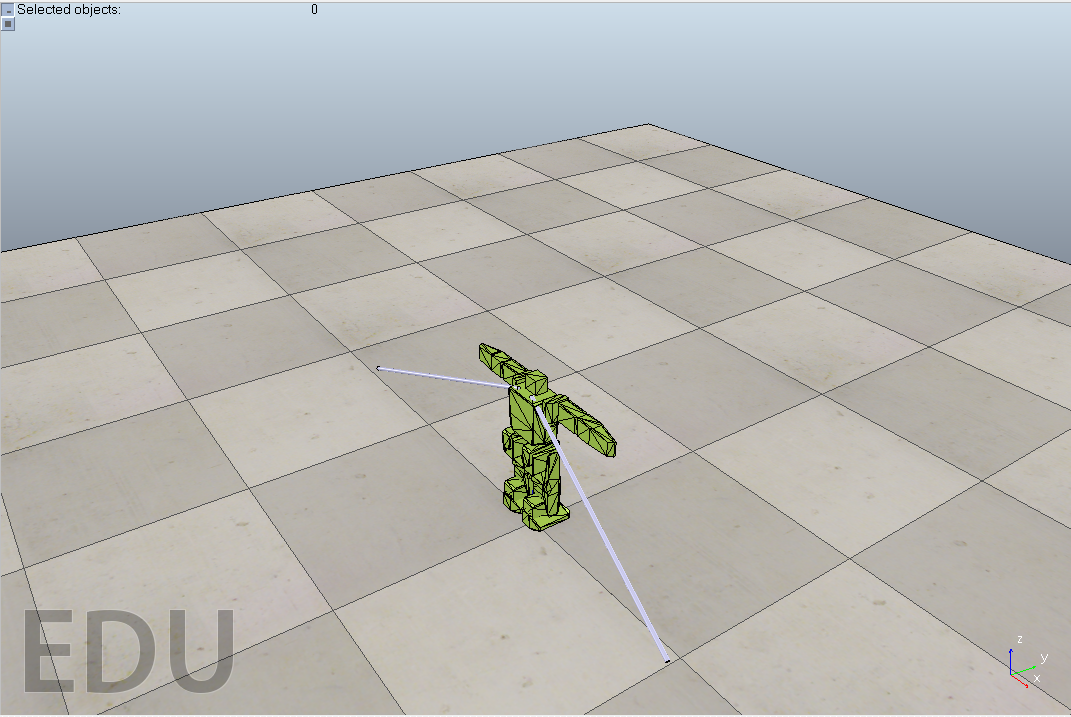
\includegraphics[width=0.35\textwidth]{include/figure/2rods.png}
    \caption{The Bioloid model with 2 support arms in the V-REP simulation enviroment.}
    \label{fig:2rods}
\end{figure}
\section{Parameters for Walking Cycle GA}
\label{app:GAparametersPrimary}
\begin{tabular}{|c|c|}
\hline
nIndividuals & 10 to 30\\
\hline
nGenerations & 50 to 70\\
\hline
pTournament & 0.75\\
\hline
pMutation & $1/genomeLength$\\
\hline
pCrossover & 0.5\\
\hline

\end{tabular}


\section{Processed Data}\label{ProcessedData}

\begin{figure}[htbp]
    \centering
    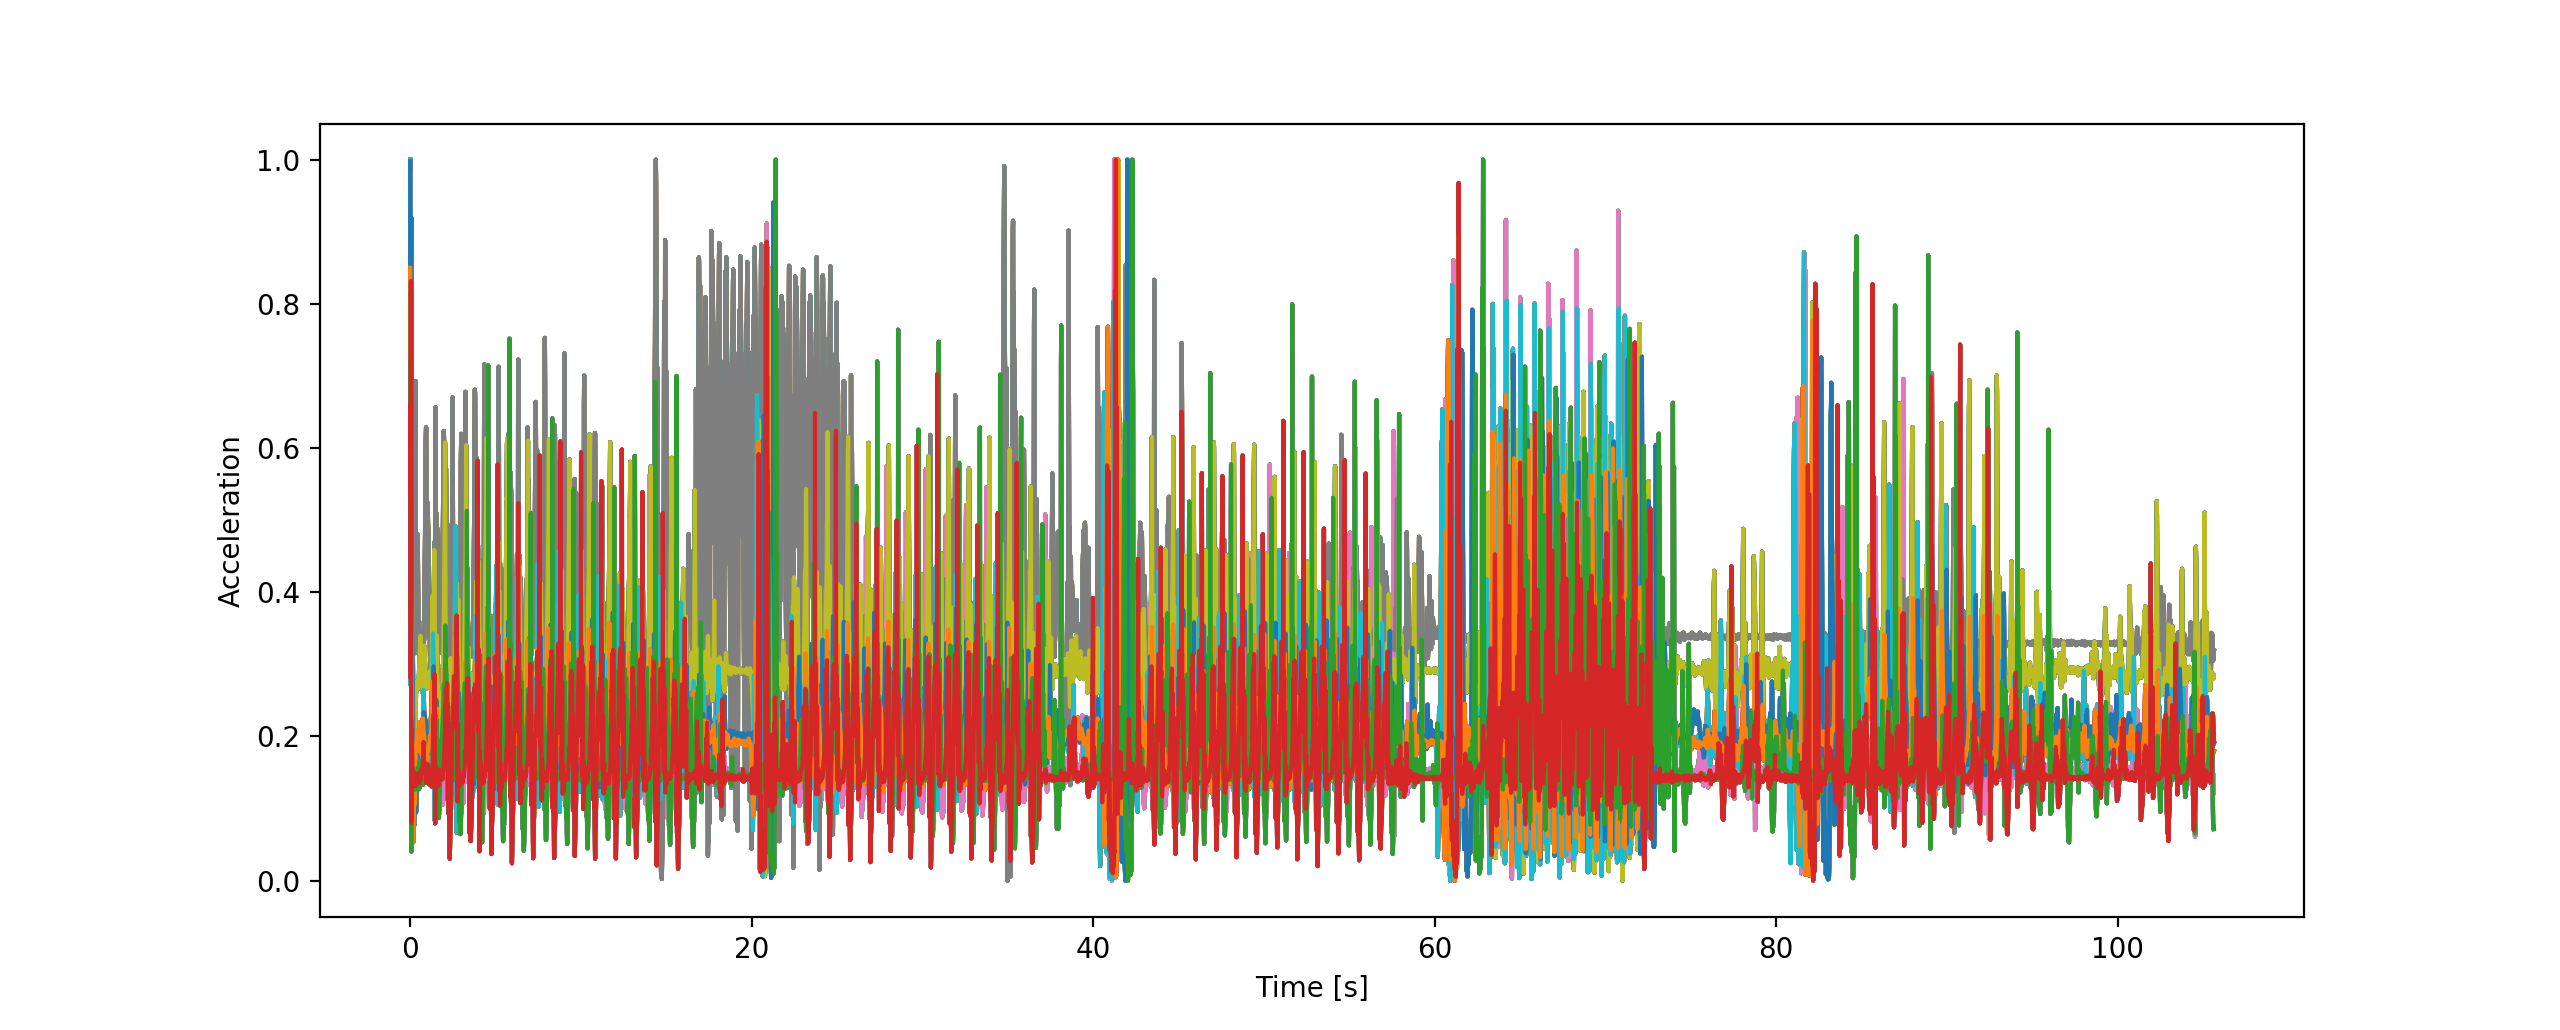
\includegraphics[width=15cm,height=8cm]
    {include/figure/AllCyc.png}
    \caption{A plot of the collected accelerometer data where the peaks represents the initilisation signals and the different colours represents the different accelerometer signals.}
    \label{fig:AllCyc}
\end{figure}

\section{Results of Pre-Evolution} \label{resultsOfPreEvolution}

\begin{figure}[htbp]
    \centering
    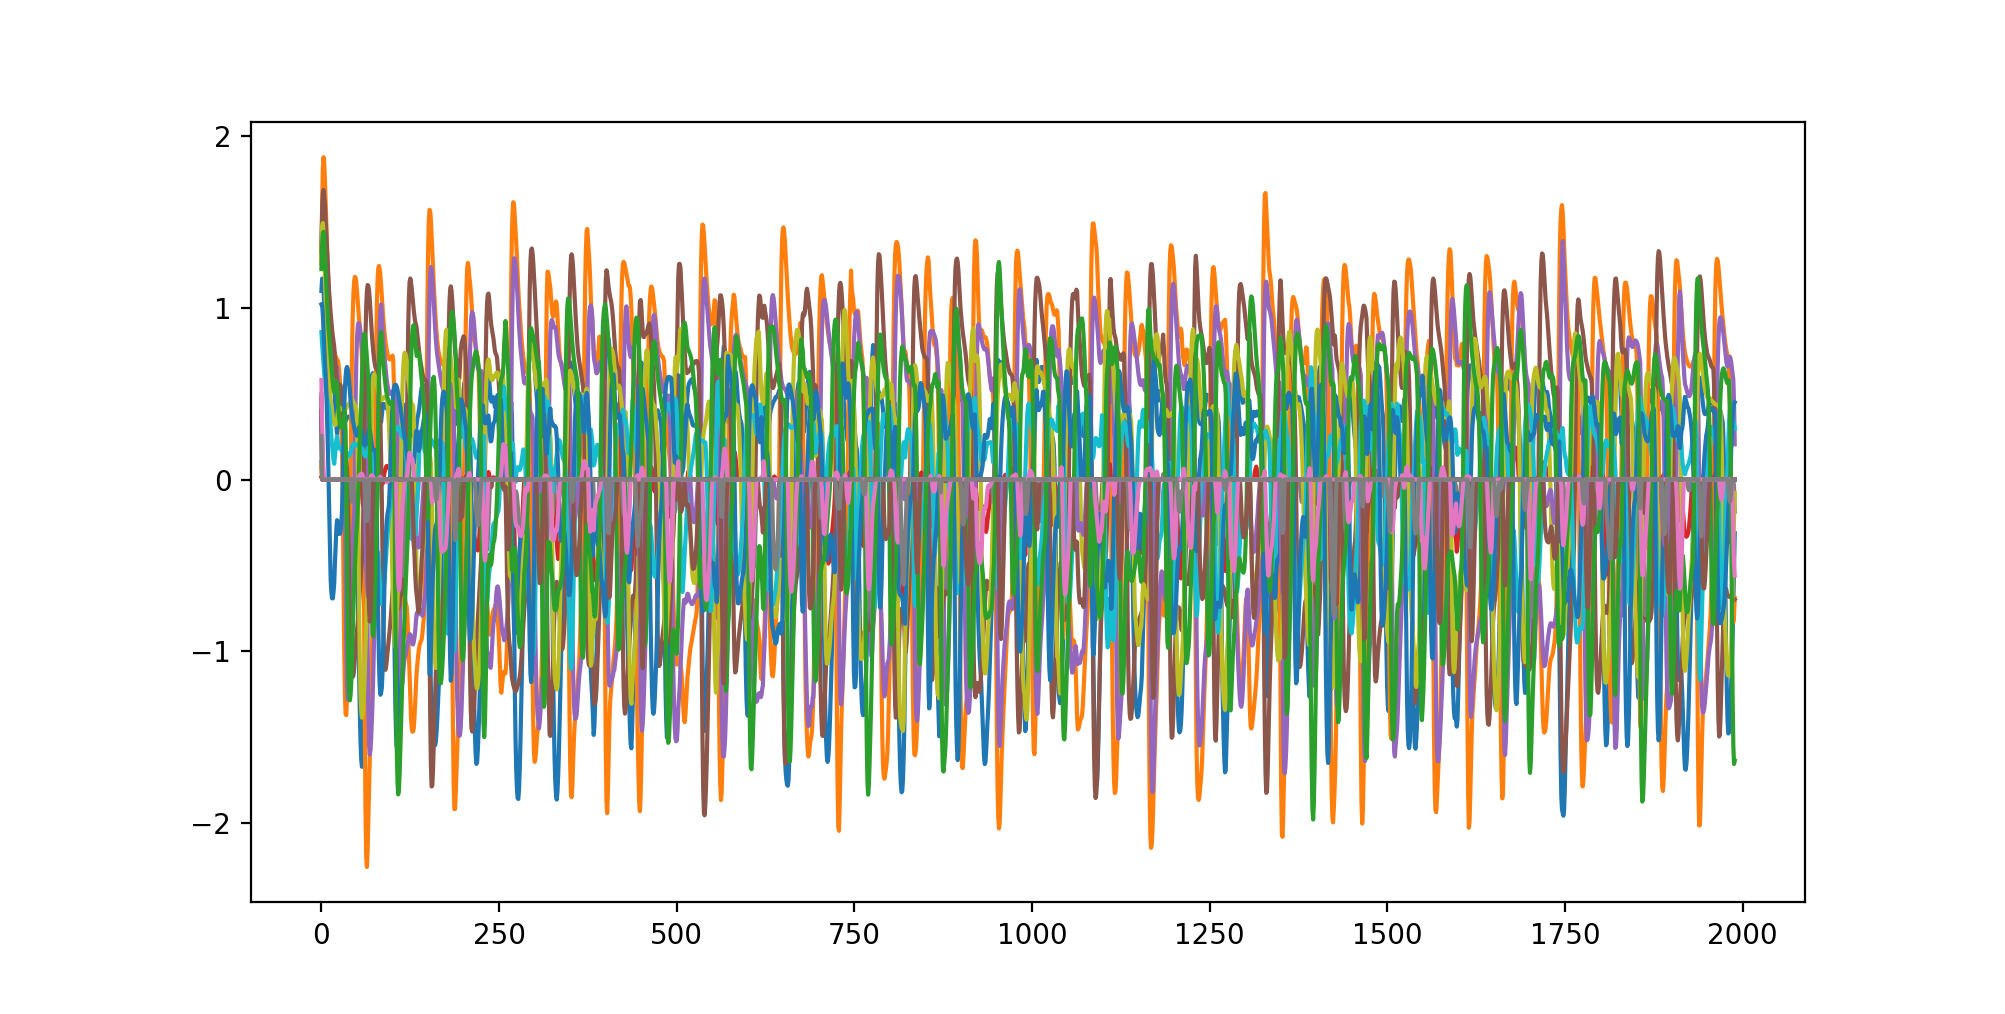
\includegraphics[width=\textwidth]{include/figure/output_500gen_w.png}
    \caption{All output signals of the best individual after 500 generations simulated. The x-axis is the simulation time, and the y-axis is the output signal represented in acceleration.}
    \label{fig:output}
\end{figure}


\begin{figure*}[t!]
    \centering
    \begin{subfigure}[b]{0.45\textwidth}
        \centering
        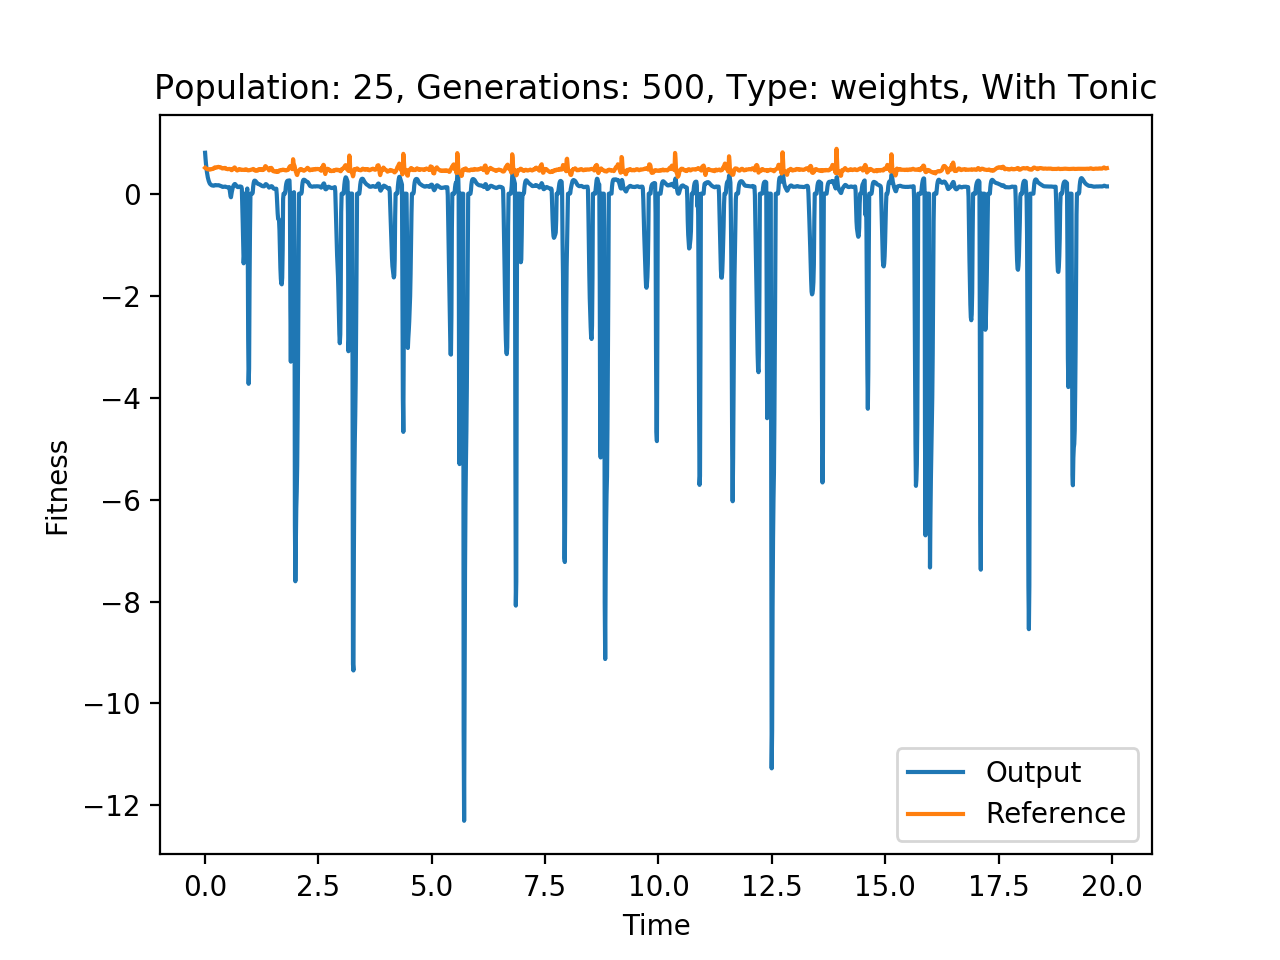
\includegraphics[width=0.95\textwidth]{include/figure/output_pop25_gen500_type0_with.png}
        \caption{Original version}
    \end{subfigure}
    ~ 
    \begin{subfigure}[b]{0.45\textwidth}
        \centering
        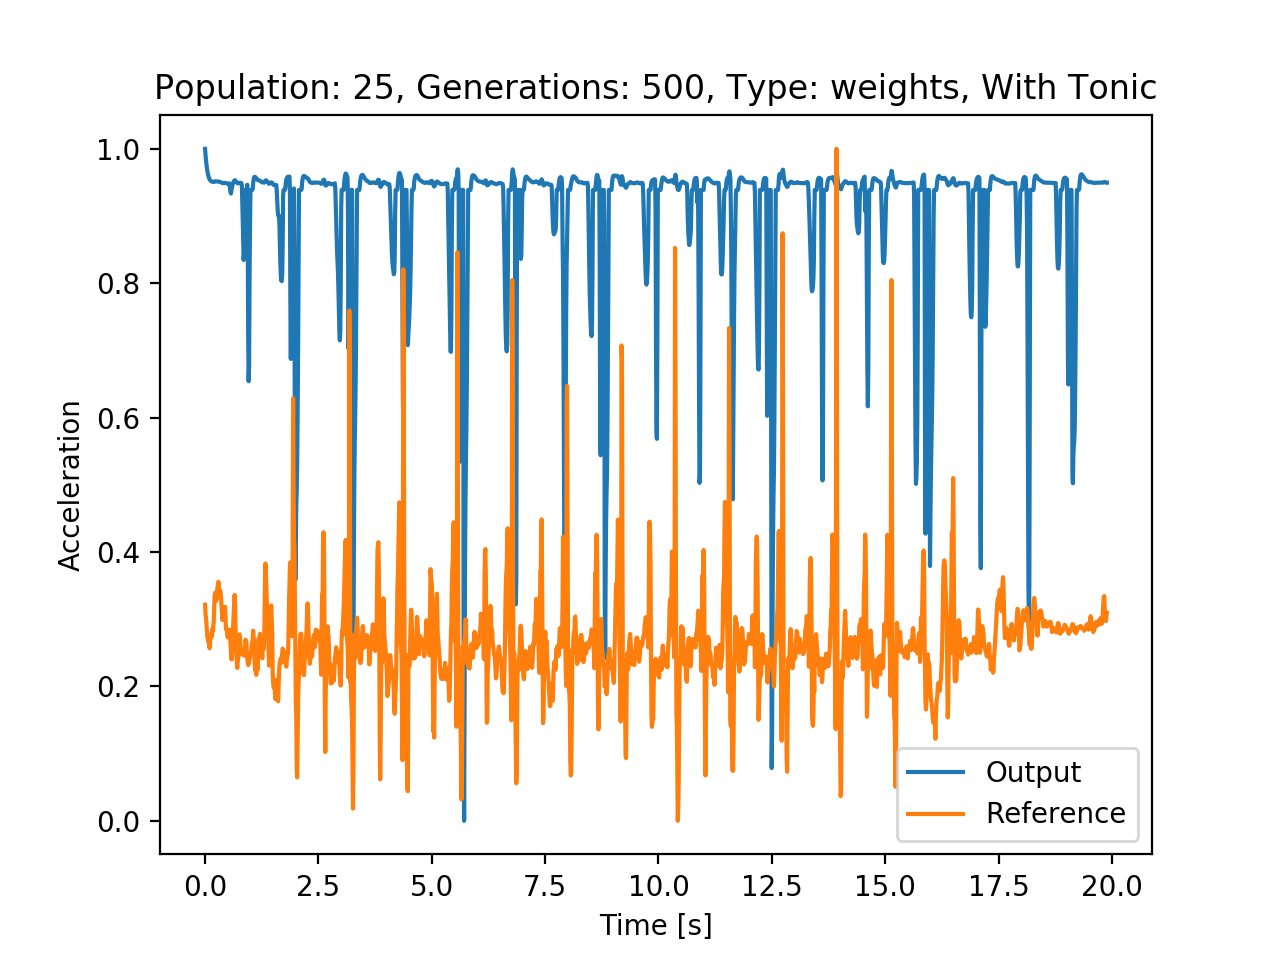
\includegraphics[width=0.95\textwidth]{include/figure/output_pop25_gen500_type0_with_normalised.png}
        \caption{Normalised version}
    \end{subfigure}%
    \caption{Output signals of the CPG network.}
    \label{fig:result_2}
\end{figure*}